\section{Evolução Arquitetural}
O processo de definição da arquitetura foi iterativo, seguindo um método de estabelecimento do modelo, validação e adequação. Para cada modelo foram analisadas as suas vantagens no cumprimento dos requisitos, bem como os seus pontos fracos, até a definição da arquitetura a ser implementada.

A primeira versão proposta baseava-se unicamente em microsserviços, responsáveis por toda a inteligência do projeto, o que a fazia interessante do ponto de vista da escalabilidade para um número muito grande de casas. Com uma arquitetura fundamentada dessa maneira, é possível a utilização transparente de quantas tecnologias forem necessárias ou desejáveis, para cada um dos serviços, sem efeitos colaterais ou impactos em outros serviços. Por outro lado, cria-se grande uma complexidade na integração entre os serviços disponíveis. A complexidade pode ser gerenciada por técnicas já consolidades, como a coreografia e a orquestração \cite{lewis}.

Com o crescimento no número de microsserviços, o \emph{overhead} para a comunicação é aumentado, visto que cada requisição necessita de um amplo número de serviços solicitados, para que possa completar a sua tarefa. Há também um uso mais intenso da infraestrutura de comunicação, já que os serviços operam por troca de mensagens, as quais sofrerão aumento proporcional ao número de chamadas. As requisições aos microsserviços devem ser autenticadas e autorizadas, conforme o requisito RNF-11, de modo que foi proposto um \emph{gateway} para os serviços da nuvem, por onde passariam todas as requisições válidas, no fluxo de comunicação com a casa. A inserção do \emph{gateway} cria um ponto único de falha, mas que pode ser evitado com técnicas de redundância e duplicação \cite{oracleSPOF}.

\begin{figure}[H]
	\centering
	\caption{Primeira versão da arquitetura do projeto Hedwig}
  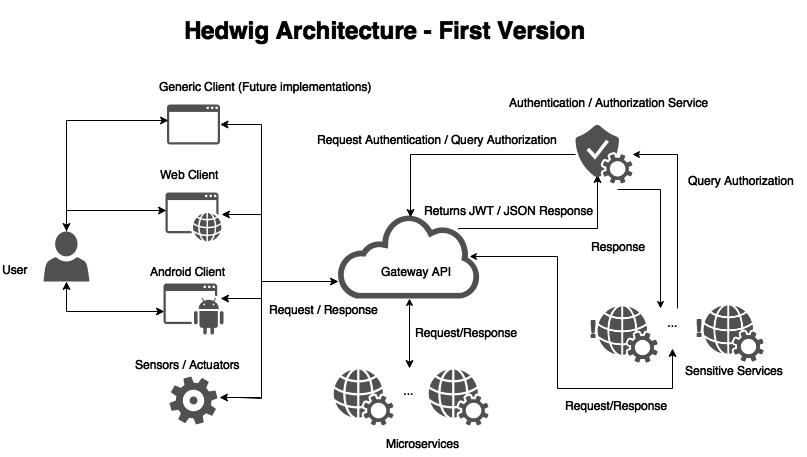
\includegraphics[width=0.9\textwidth]{arquiteturaV1}
\label{fig:arquiteturaV1}
\end{figure}

É possível observar que alguns microsserviços são classificados como sensitivos, os quais dependem de nova consulta ao serviço de autenticação e autorização para garantir a segurança. Esses serviços são todos aqueles responsáveis por tomar uma ação em relação à casa que envolva riscos, como a abertura de portões. Os microsserviços não-sensitivos utilizam a autenticação já realizada pelo \textit{gateway} na chegada da requisição.

Quando uma requisição chega à nuvem, ela deve ser validada, para garantir a sua origem (RNF-11), e o método adotado faz uso de \emph{tokens}.  Caso passe nos critérios de autenticação e autorização, é retornado um JWT (\textit{JSON Web Token}), necessário para os passos seguintes. O JWT é discutido na seção \ref{sec:JWT}.

De extrema importância, e não cobertos pela arquitetura anterior, são os requisitos de disponibilidade do projeto (RNF-4). Se o \textit{gateway} estiver inacessível em determinado momento, a casa não terá mais nenhuma forma de comunicação com os meios externos, mesmo para os serviços mais básicos. Para resolver este problema, foi proposta uma segunda versão, conforme ilustra a imagem seguinte.

\begin{figure}[H]
	\centering
	\caption{Segunda versão da arquitetura do projeto Hedwig}
  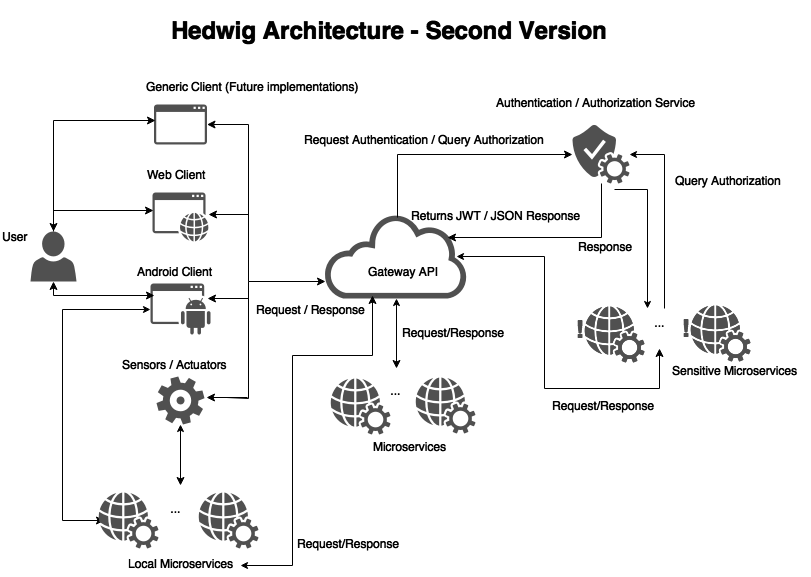
\includegraphics[width=0.9\textwidth]{arquiteturaV2}
\label{fig:arquiteturaV2}
\end{figure}

Nesta versão, serviços essenciais seriam duplicados dentro da casa e, no caso de haver qualquer forma de impedimento na comunicação com a nuvem, esses serviços seriam responsáveis por controlar diretamente os atuadores desejados. Entretanto, cria-se mais uma complexidade ao manter serviços duplicados na casa, e no caso destes serviços também não estarem online no momento necessário, novamente não seriam alcançados requisitos de disponibilidade. Contudo, é uma versão que chega mais próxima de obedecer às necessidades do projeto.

Essa arquitetura provê módulos sem inteligência, e todo o controle é feito pelo serviço correspondente. Essa escolha desfruta de benefícios como a escalabilidade, a manutenção (já que é extremamente mais simples atualizar o software nos servidores do que nas residências) e a facilidade para prover correções ou possíveis aumentos de funcionalidade. Entretanto, alguns módulos poderiam ficar em lugares de difícil acesso --- ou mesmo fora da casa --- onde a comunicação poderia ser intermitente ou mesmo perdida. Assim, em caso de falha de comunicação, um atuador não receberia os sinais necessários do serviço, acarretando em sérios problemas na proteção da casa. No caso de uma garagem, por exemplo, o portão permaneceria aberto indeterminadamente, ou poderia não ser aberto quando o morador chegasse em sua casa.

Assim, avançou-se para o desenvolvimento de um modelo arquitetural modularizado, onde cada módulo teria inteligência para realizar as tarefas necessárias e, ao mesmo tempo, poderia enviar dados à nuvem e ser avisado quando for necessário realizar uma tarefa. Além disso, no aspecto comercial, módulos inteiros poderiam ser vendidos, substituídos e aumentados.

A arquitetura projetada faz uso de microsserviços no lado da nuvem e, no lado da casa, os componentes de hardware passam a ser agrupados em módulos independentes, com responsabilidades bem estabelecidas (RNF-1), inteligência e autonomia para realizar todas as atividades necessárias. Os módulos se comunicarão com um servidor local, que realizará, por último, a conexão direta com os serviços não locais. Esse servidor se comunicaria com os módulos por meio de mensagens enviadas em tópicos, as quais seriam interpretadas e enviadas aos servidores remotos em canais protegidos (RNF-2). O requisito RNF-8, relativo à escalabilidade, não será verificado no projeto, e pode ser considerado em passos futuros.

Em uma eventualidade, a comunicação entre o servidor local e a nuvem pode ser perdida.  O usuário, no entanto, deve conseguir se comunicar com a casa, ainda que tenha ao seu dispor uma quantidade mais restrita e essencial de ações --- como a liberação de acesso à casa. Quando é perdida a conexão entre a casa e os serviços externos, o servidor local armazena as mensagens vindas dos módulos, que serão transmitidas ao servidor remoto posteriormente. Como não há urgência para o processamento de tais dados (visto que não são requisições de ações, mas comunicação de estado) --- os quais serão utilizados para análise de comportamento e aprendizado de máquina (RF-5) --- não há prejuízo com o eventual envio tardio. O usuário poderá acompanhar o estado da casa, com as informações vindas dos sensores, por meio de um segundo aplicativo, denominado aplicativo backup.

No caso mais extremo, de perda de comunicação tanto com a nuvem quanto com o servidor local, como na ocorrência de falha de hardware do servidor local, os dados que os módulos tentam enviar ao servidor local serão perdidos, entretanto o aplicativo backup continua podendo se comunicar diretamente com os módulos, para ter acesso aos serviços de extrema importância.
